\subsection{Jet deflection}
The most direct way to measure the structure of matter is the controlled scattering of a beam of probe particles. This approach was used to discover the atomic nucleus and quarks and gluons, and it is employed today to explore the partonic structure of nucleons and nuclei. The partonic phase of the QGP lives for $\sim10^{-23}$ seconds before breaking up into hadronic remnants, so that probing it by the scattering of an externally-generated beam is impossible in practical terms. 

As an alternative, energetic jets arising from high-$Q^2$ processes in the same nuclear collision that generates the QGP provide internally-generated probes that may be applied for this purpose (refs Bjorken, Gyulassy+Pluemer, Gyulassy+Wang, Salgado+Wiedemann, BDMPS). Study of the interaction of jets with the QGP (``jet quenching'') is a central focus of the LHC heavy ion program, and projections for jet quenching observables in Run 3/4 are discussed extensively in this chapter. In this section we discuss the most direct jet probe of the QGP: the angular deflection of the jet relative to its initial direction due to momentum transfer with the medium. 

Jet deflection can only be measured by coincidence observables, in which an axis is determined by a trigger object, and the deflection of the jet recoiling from the trigger is measured relative to that axis. Such scattering measurements, carried out over a wide range in energy and resolution scale, can be used to explore the microscopic structure of the QGP. For instance, modification in the rate of rare, large-angle jets in nuclear collisions relative to a vacuum reference may arise from the scattering off quasi-particles of the QGP, thereby probing their nature~\cite{DEramo:2012uzl}. In addition, the recoil distribution at small recoil jet angles relative to $\pi$ may be modified by soft in-medium multiple scattering, which can provide a direct measurement of the jet transport parameter \qhat~\cite{Chen:2016vem}.

Measurements of the angular distribution of jets relative to a trigger axis have been reported for di-jet, gamma-jet, and hadron-jet coincidences, at both RHIC~\cite{Adamczyk:2017yhe} and LHC ~\cite{Adam:2015doa} (add refs for ATLAS/CMS di-jet and gamma+jet acoplan). These current measurements exhibit no evidence of in-medium modification of angular distributions, both at small and large angles to the trigger axis. While they impose initial constraints on the magnitude of in-medium scattering effects, their statistical and systematic precision are limited. Measurements in LHC Run3/4 will either discover in-medium modification to the recoil jet angular distributions, or improve these constraints substantially.

Jets are complex dynamical objects. The shower of an energetic jet develops over an extended time interval, with the decoherence time of radiation in the shower  correlated with its hardness and angle~\cite{Andrews:2018jcm}. Jet quenching arises from modification of this radiation pattern, due to scatterings with quarks and gluons in the medium and the quantum-mechanical interference between medium-induced and vacuum processes~\cite{Andrews:2018jcm} (other refs?). The picture of in-medium angular deflection of a jet, as described above, corresponds to coherent scattering of a highly virtual parton prior to development of the jet shower. However, deflection of a decohered branch of the shower can also occur~\cite{DEramo:2018eoy}, resulting in both broadening of the jet shower and overall deflection of the jet centroid. 

There is an intensive ongoing effort to develop analysis tools and calculational approaches that discriminate the various contributions to in-medium jet deflection and shower modification, in both experiment and theory~\cite{Andrews:2018jcm} (ref to other sections in this report). In this section we focus solely on jet-centroid deflection measurements, without consideration of the effects of shower broadening or other shower modification (see Sect XXX). Measurements of both classes of jet quenching observable must ultimately be interpretable in a single consistent picture, but such an approach is beyond current experimental and theoretical capabilities.

The most significant background to the measurement of medium-induced jet deflection is broadening of the recoil angular distribution due to well-established vacuum QCD effects, in particular Sudakov radiation, which is soft radiation outside the jet cone that generates a broad peak in the recoil jet angular distribution relative to the trigger axis~\cite{Chen:2016vem,Mueller:2016xoc}. Angular broadening due to Sudakov radiation grows with $\sqrt{s}$, and with jet energy; from this standpoint, relatively low energy jets are preferable to minimize this background~\cite{Chen:2016vem}.

The largest in-medium jet deflection effects are likewise expected for relatively low-energy jets, which experience the largest angular deflection from a given momentum transfer between the jet and medium~\cite{DEramo:2018eoy,Gyulassy:2018qhr}. In addition, a model calculation of a jet interacting with a static QGP ``brick" at fixed temperature indicates that medium-induced large-angle radiation relative to the jet axis arises predominantly from partons from the medium that are scattered by the jet, with a resulting momentum spectrum that is significantly softer than the in-vacuum recoil jet spectrum~\cite{DEramo:2018eoy}. Another recent calculation, that includes the effects of vacuum Sudakov radiation and jet-medium interactions based on the few-hard (GLV) or multiple-soft (BDMPS) scattering approaches to jet quenching, finds that the acoplanarity distributions for these different jet quenching pictures differ by a few percent in the range $20<\ptjet<40$ \gevc~\cite{Gyulassy:2018qhr}. This sets the precision required for definite jet-scattering measurements in Run 3/4. Additional theoretical considerations of in-medium \pT-broadening can be found in \cite{Zakharov:2018rst,Ghiglieri:2018ltw}.

In light of such considerations, it is necessary to utilize analysis techniques that can attain $\sim$few percent precision in the measurement of recoil jet angular distributions for low \ptjet\ and large jet radius $R$, over the large and complex uncorrelated backgrounds in central \PbPb\ collisions at the LHC. This precision is achievable using the statistical approach to jet background correction~\cite{Adam:2015doa,Adamczyk:2017yhe}, in which the discrimination of trigger-correlated and uncorrelated recoil jet yield is carried out in a fully data-driven way, at the level of ensemble-averaged distributions. The statistical correction approach has been used to measure the azimuthal distribution for charged jets with $R=0.5$ and $40<\ptjetch<60$ \gevc\ recoiling from a high-\pt\ hadron in central \PbPb\ collisions at the LHC~\cite{Adam:2015doa}, and for charged jets with $R=0.5$ and $\ptjetch\sim10$ \gevc\ in central \AuAu\ collisions at RHIC~\cite{Adamczyk:2017yhe}. We expect that the latter is likewise achievable at the LHC, with good systematic precision. 

The required experimental approach is therefore in hand, and we explore here the statistical precision achievable using it for such measurements in Run 3/4. 
We utilize the JEWEL model (ref) for these projections. {\it (The physics content of JEWEL will certainly be described elsewhere in this chapter, insert pointer here.)} Calculations are carried out for central \PbPb\ collisions at \sqrtsnn{5.02} with integrated luminosity of 10 nb$^{-1}$ , and \pp\ collisions at \sqrts{5.02} with integrated luminosity of 6 pb$^{-1}$. 

The JEWEL calculations for central \PbPb\ collisions are carried out with the ``Recoil off" configuration. As noted in ~\cite{DEramo:2018eoy}, large-angle jet yield at low \ptjet\ may be dominated by the scattering of partons that originated in the medium. While quantitative exploration of this effect is beyond the scope of this initial calculation, we expect that the ``Recoil on" configuration of JEWEL will generate larger yields due to in-medium scattering than we report below.

%----------
\begin{figure}[tbh!]
\centering
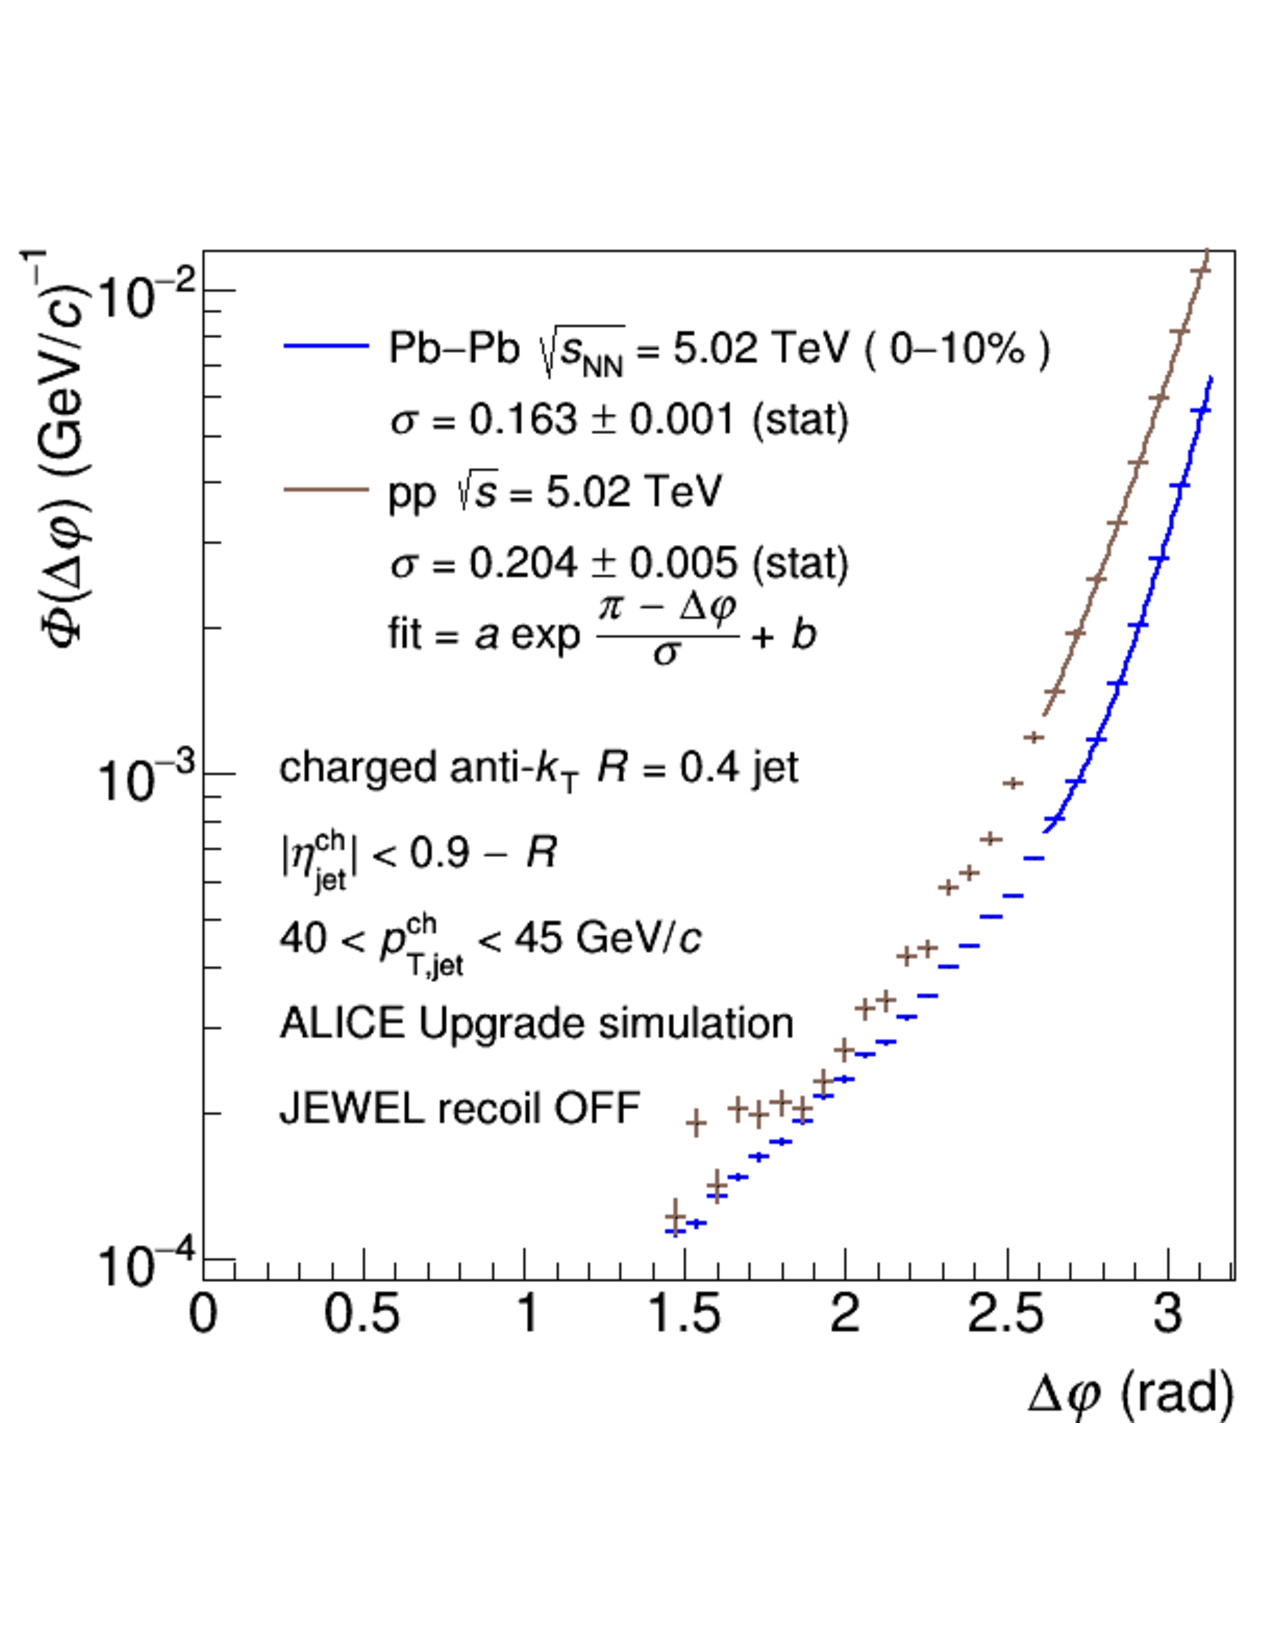
\includegraphics[width=0.6\textwidth]{figures/jetdeflection/JetDeflectionFig_Phi.pdf}
\caption{JEWEL simulation of the angular distribution of charged jet yield in the ALICE acceptance for  $40<\ptjetch<45$ \gevc\ and $R=0.4$ recoiling from a high-\pt\ trigger hadron ($20<\ptt<50$ \gevc), for central \PbPb\ collisions at \sqrtsnn{5.02} with 10 nb$^{-1}$ int. lumi, and \pp\ collisions at \sqrts{5.02} with 6 pb$^{-1}$ int. lumi. The recoil jet azimuthal angle \Dphi\ is defined with respect to the trigger axis. The observable shown is $\Phi(\Dphi)$, defined in~\cite{Adam:2015doa}, which incorporates statistical suppression of uncorrelated background.
}
\label{fig:JetDeflectionPhi}
\end{figure}
%----------

Figure~\ref{fig:JetDeflectionPhi} shows a JEWEL simulation of $\Phi(\Dphi)$~\cite{Adam:2015doa}, the background-corrected azimuthal distribution of recoil jets recoiling from a high-\pT\ trigger hadron, with the statistics expected by ALICE for central \PbPb\ and \pp\ collisions in Run 3/4. The distribution for central \PbPb\ collisions exhibits an overall yield suppression, corresponding to jet quenching, but also a slight narrowing of the main peak at $\Dphi\sim\pi$ and an enhancement at large deflection angle. JEWEL evidently predicts significant transport of recoil jet yield away from the trigger axis.

%----------
\begin{figure}[tbh!]
\centering
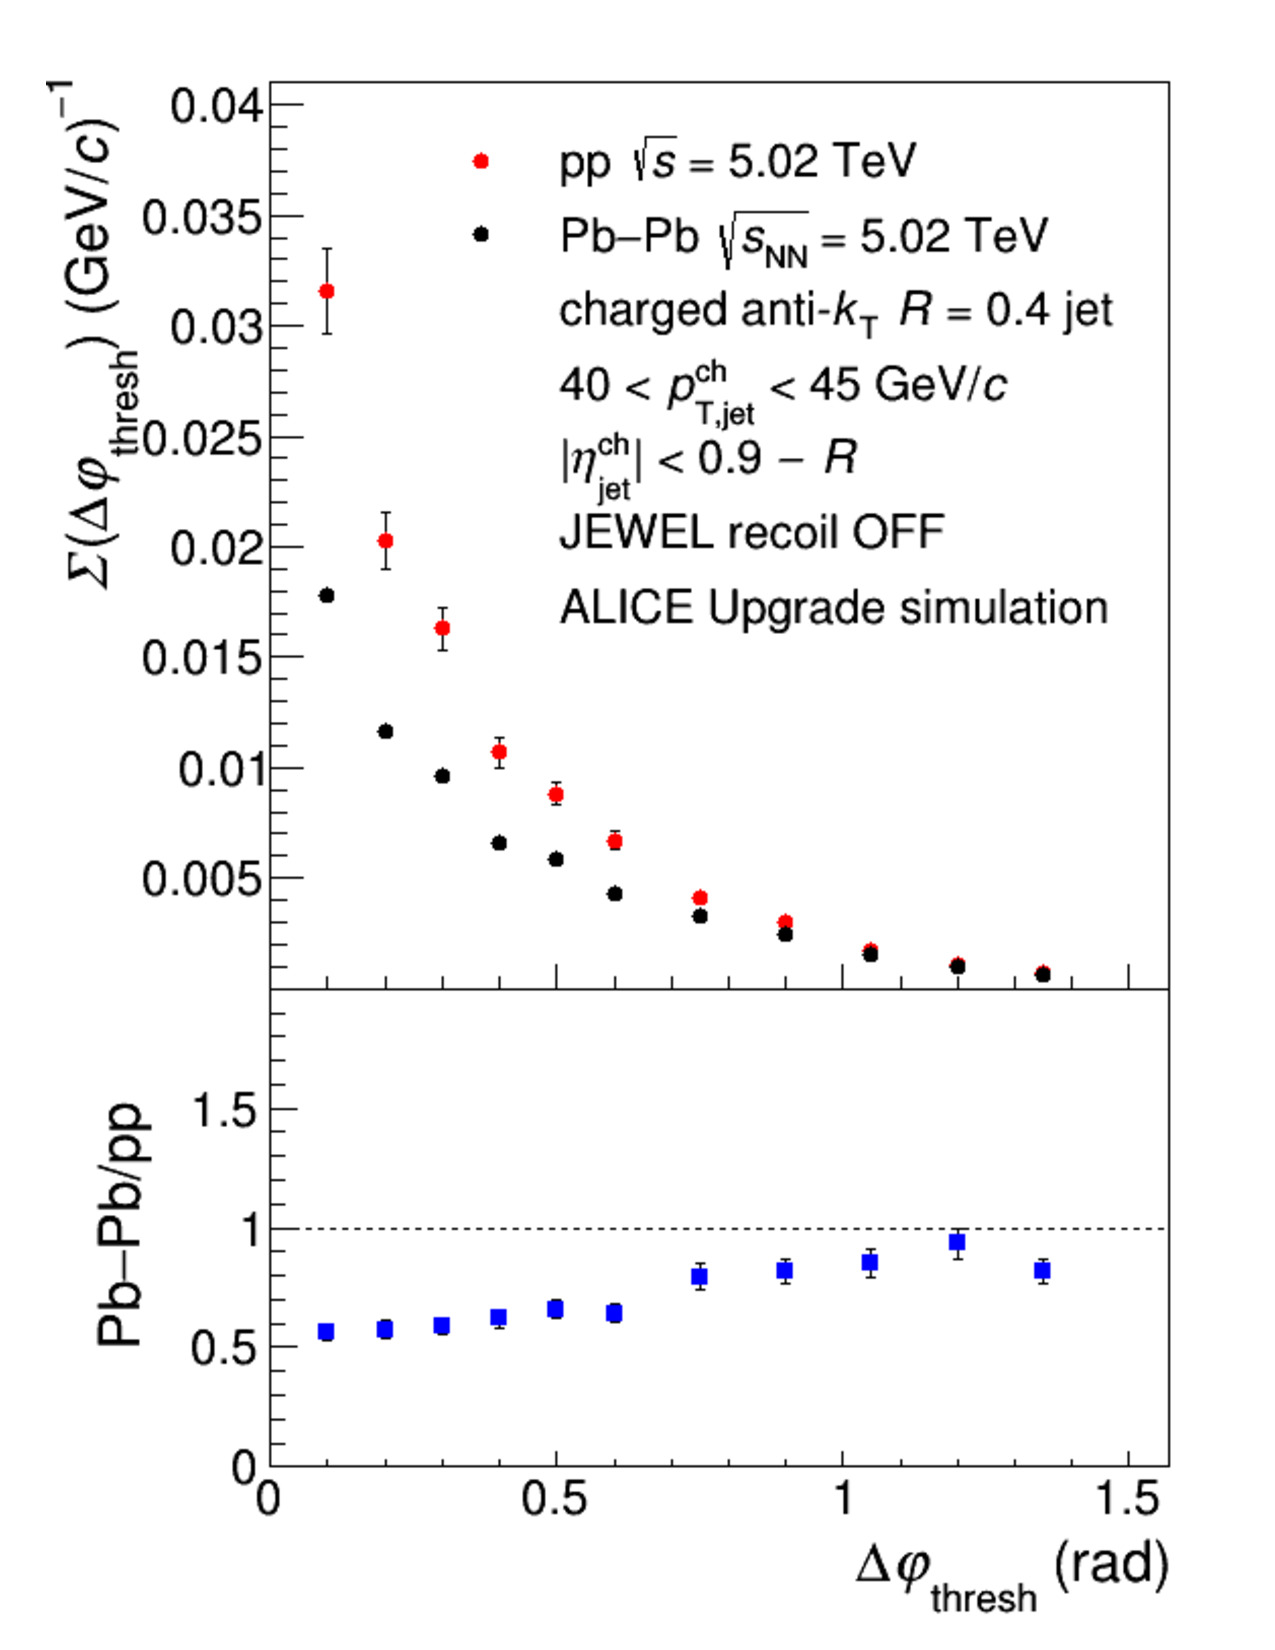
\includegraphics[height=0.6\textwidth]{figures/jetdeflection/JetDeflectionFig_Sigma.pdf}
\caption{Cumulative large-angle yield $\Sigma(\dphithresh)$ (Eq.~\ref{eq:Sigma}) vs. \dphithresh\ for the \pp\ and central \PbPb\ distributions $\Phi(\Dphi)$ in Fig.~\ref{fig:JetDeflectionPhi}. See text for details. 
}
\label{fig:JetDeflectionSigma}
\end{figure}
%----------

In order to quantify the difference at large recoil jet deflection angle between \pp\ and central \PbPb\ collisions, we integrate the $\Phi(\Dphi)$ from $\pi/2$ to a threshold angle \dphithresh~\cite{Adam:2015doa},

\begin{equation}
\Sigma(\dphithresh) = 
\int_{\pi/2}^{\pi-\dphithresh}
\Phi(\Delta\varphi)\mathrm{d}\Delta\varphi.
\label{eq:Sigma}
\end{equation}

\noindent
Figure~\ref{fig:JetDeflectionSigma} shows $\Sigma(\dphithresh)$ for the $\Phi(\Dphi)$ distributions in Fig.~\ref{fig:JetDeflectionPhi}, together with their ratio. In this calculation, the value of $\Sigma$ at $\dphithresh=0$ is around 0.5, which is the yield suppression averaged over the full recoil hemisphere. The ratio grows to $\Sigma\sim1$ at $\dphithresh=1.2$, indicating a factor two enhancement in large-angle yield relative to the hemisphere average. The statistics of the measurement are clearly sufficient to measure the effect predicted by this calculation.

However, the calculation in~\cite{Gyulassy:2018qhr} predicts a difference of only a few percent in these distributions for GLV-like and BDMPS-like in-medium scattering, which is more difficult to discriminate. The statistical error in the ratio in Fig.~\ref{fig:JetDeflectionSigma} is around 5\% at $\dphithresh\sim1$, due predominantly to the statistical precision of the \pp\ distribution. Improvement in the statistical precision of this measurement, needed to achieve $\sim$percent absolute precision, requires larger integrated luminosity for the \pp\ dataset than the value of 6 pb$^{-1}$ used for this calculation.

As in Sect.~\ref{sect:JetQuenchSmallSys}, we do not discuss here projections for systematic uncertainties of the jet deflection measurement, since such uncertainties depend crucially on {\it in-situ} detector performance and other factors that are not presently known. We note, however, that the precision of the current jet deflection measurements at low \ptjetch, carried out using the statistical background correction approach, is strongly dominated by statistical error ~\cite{Adam:2015doa,Adamczyk:2017yhe}, and that significant improvement in systematic uncertainties is expected for Run 3/4 relative to these initial measurements.  

